\documentclass[12pt]{article}
\usepackage{graphicx}
\usepackage{amsmath}
\usepackage{mathtools}
\usepackage{gensymb}

\newcommand{\mydet}[1]{\ensuremath{\begin{vmatrix}#1\end{vmatrix}}}
\providecommand{\brak}[1]{\ensuremath{\left(#1\right)}}
\providecommand{\norm}[1]{\left\lVert#1\right\rVert}
\providecommand{\abs}[1]{\left\vert#1\right\vert}
\newcommand{\solution}{\noindent \textbf{Solution: }}
\newcommand{\myvec}[1]{\ensuremath{\begin{pmatrix}#1\end{pmatrix}}}
\let\vec\mathbf

\begin{document}
\begin{center}
\textbf\large{CONIC SECTIONS}

\end{center}
\section*{Excercise 11.5}
Q8.An equilateral triangle is inscribed inthe parabola $y^2 = 4ax$, where one vertex is at the vertex of the parabola. Find the length of the side of the triangle.

\solution
The given equation of the parabola can be rearranged as
\begin{align}
	\label{eq:eq1}
	y^2-4ax=0
\end{align}
The above equation can be equated to the generic equation of conic sections
\begin{align}
	\label{eq:eq2}
	g\brak{\vec{x}}=\vec{x}^\top \vec{V}\vec{x}+2\vec{u}^\top \vec{x}+f=0
\end{align}
Comparing the coefficients of both equations \eqref{eq:eq1} and \eqref{eq:eq2}
\begin{align}
	\label{eq:eqV}
	\vec{V} &= \myvec{0&0\\0&1}\\
	\label{eq:eqU}
	\vec{u} &= -\myvec{-2a\\0}\\
	\label{eq:eqF}
	f &= 0
\end{align}
Let length of side of triangle = r.
Since,triangle is inscribed in the parabola and one of the vertex of the triangle lies at the vertex of the parabola, the other vertices are given as
\begin{align}
	\label{eq:eq3}
	\vec{P} &= \myvec{r\cos 30\degree\\r\sin 30\degree} = \myvec{\frac{\sqrt{3}}{2}r\\\frac{1}{2}r}\\
	\vec{Q} &= \myvec{r\cos 30\degree\\-r\sin 30\degree} = \myvec{\frac{\sqrt{3}}{2}r\\-\frac{1}{2}r}
\end{align}
Now these point will satisfy the equation of the parabola. So substituting \eqref{eq:eq3} in \eqref{eq:eq2}
\begin{align}
	\vec{P}^\top \vec{V}\vec{P}+2\vec{u}^\top \vec{P}+f&=0\\
	\myvec{\frac{\sqrt{3}}{2}r&\frac{1}{2}r}\myvec{0&0\\0&1}\myvec{\frac{\sqrt{3}}{2}r\\\frac{1}{2}r}+2\myvec{-2a&0}\myvec{\frac{\sqrt{3}}{2}r\\\frac{1}{2}r} &= 0\\
	\frac{1}{4}r^2 - 2a\sqrt{3}r &= 0\\
	r\brak{\frac{r}{4} - 2a\sqrt{3}} &= 0
\end{align}
Hence, the length of side of triangle is
\begin{align}
	r &= 8a\sqrt{3}
\end{align}
The result will be the same for substituting $\vec{Q}$. See Fig.\ref{fig:Fig1}.
\begin{figure}[!h]
	\begin{center} 
	    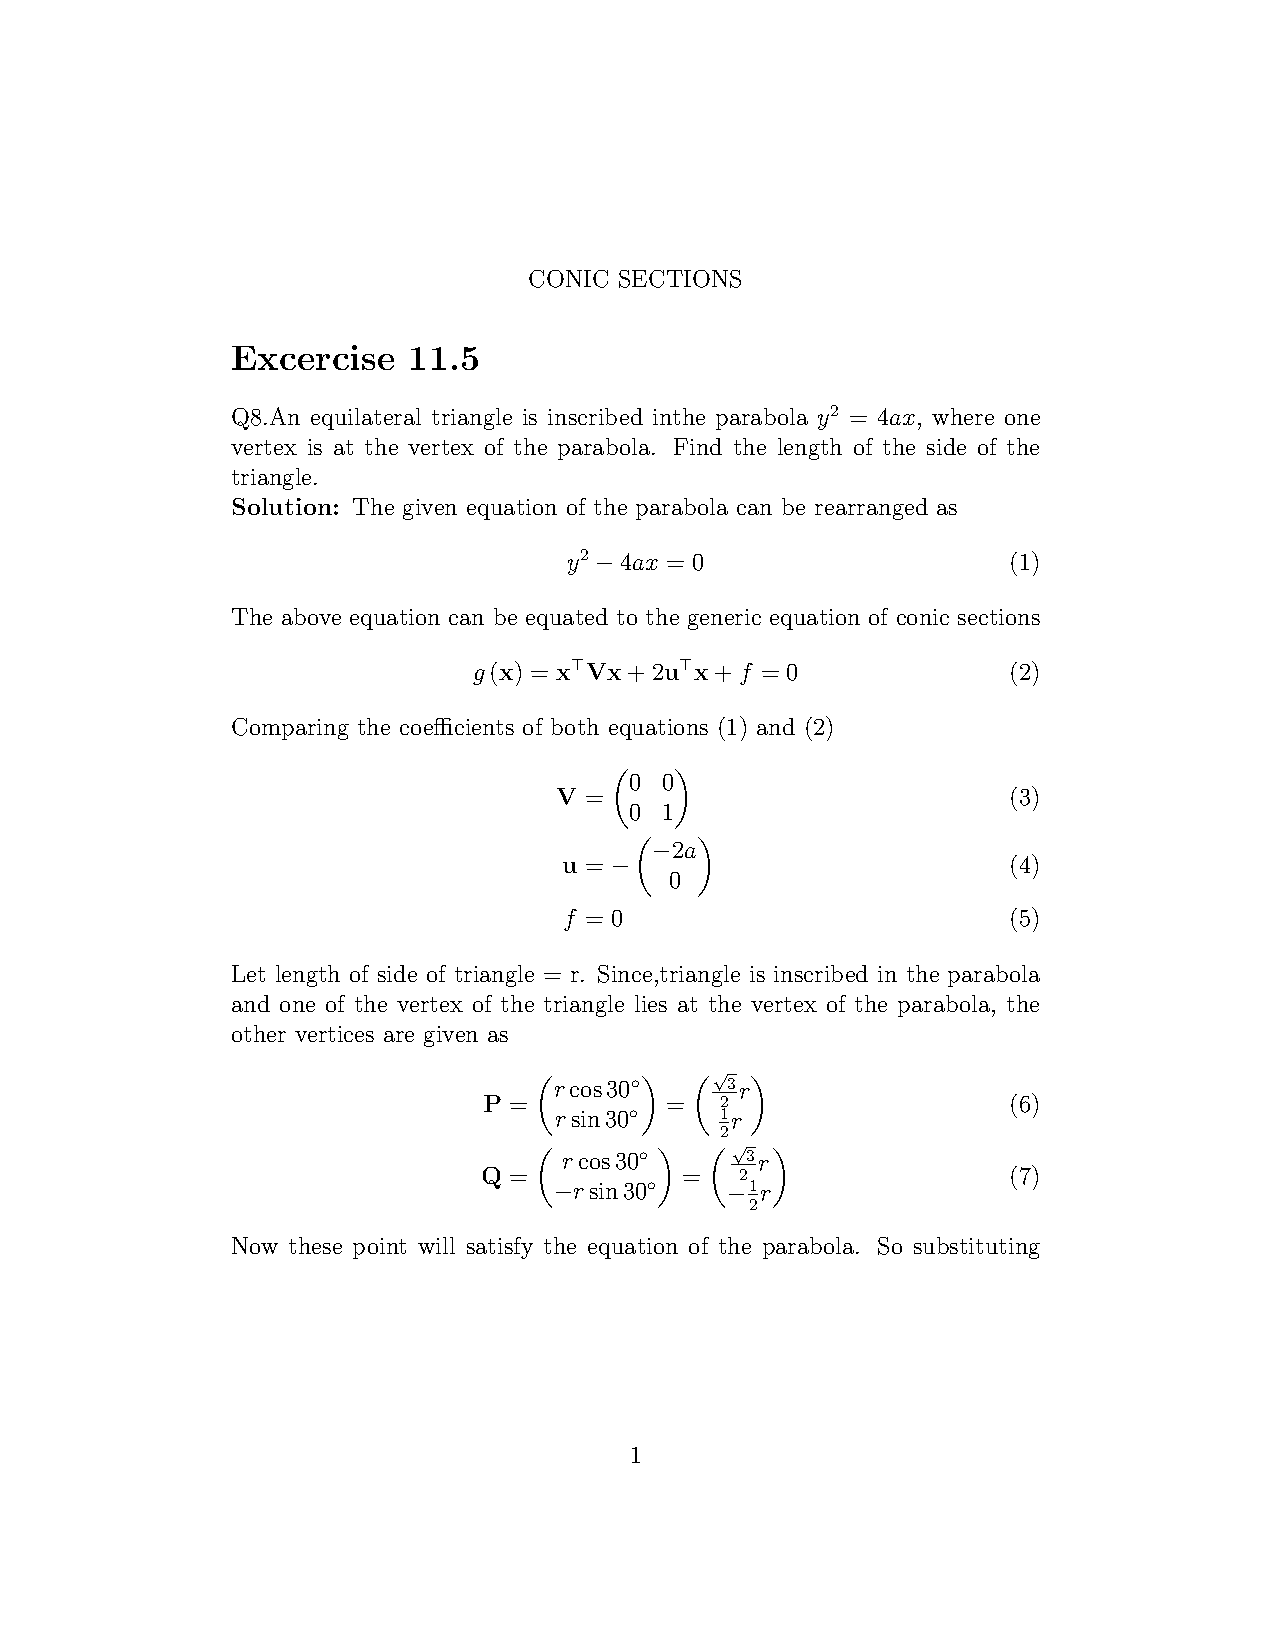
\includegraphics[width=\columnwidth]{figs/conic5}
	\end{center}
\caption{}
\label{fig:Fig1}
\end{figure}

\end{document}
